Recent work has begun to explore how autoregressive (AR) and diffusion-based language models (DLLMs) can learn from one another, yielding improvements in sample efficiency, quality, and alignment.  

This section examines bidirectional knowledge transfer between these paradigms, focusing on distillation techniques that enable DLLMs to leverage AR model expertise, as well as hybrid approaches that incorporate diffusion mechanisms into AR frameworks.
\begin{figure*}[h!]
    \centering
    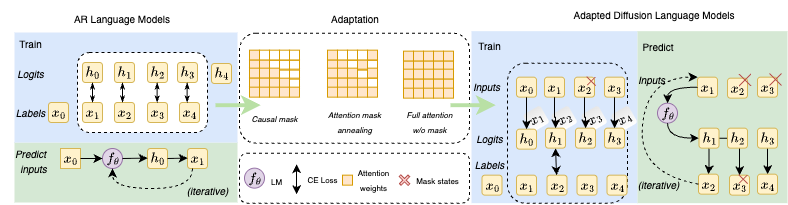
\includegraphics[width=0.95\textwidth]{figs/Adaptation/adaptation.png}
    \caption[Adaptation of AR models to diffusion models]{%
        The overview of Gong et al.'s~\cite{gong_scaling_2025} approach to adapt autoregressive (AR) models to diffusion models. 
        \textbf{Left}: The shift operation in AR models enables the output layer $h_i$ to approximate the distribution of next tokens $x_{i+1}$ in hidden representations through the cross entropy (CE) loss. 
        \textbf{Middle}: Gradually removing the causal mask during training eventually makes the model bidirectional. 
        \textbf{Right}: Inside the diffusion models, shifting the logits to compute the loss with the next token (i.e., the loss on $h_i$ would be concerning $x_{i+1}$), while perceptually, the diffusion models are still functioning as recovering the original signals (since $h_i$ corresponds to $x_{i+1}$ in AR loss).%
    }
    \label{fig:adaptation_overview}
\end{figure*}

% 对于 DLLMs 训练,来自 AR 模型的知识迁移可以作为缓解其历史较短和投资少于 AR 对应物的手段
For DLLM training, knowledge transfer from AR models can mitigate the challenges arising from their shorter development history and reduced investment compared to their AR counterparts. % DLLMs 可以从 AR 模型中蒸馏,就像较小的 AR 模型从较大的模型中逐令牌蒸馏一样
DLLMs can be distilled from AR models using the same token-by-token approach employed when distilling smaller AR models from larger ones. % Gong 等人在《通过自回归模型适应扩展扩散语言模型》中表明
Gong et al. present a method to in \textbf{Scaling Diffusion Language Models via Adaptation from Autoregressive Models}. Their approach first initializes the diffusion model's noise schedule and attention masks based on a pretrained AR checkpoint. Then the model is then fine-tuned with a combination of denoising and next-token prediction losses. The resulting DLLM inherits both the global coherence and fast convergence properties of the teacher AR model while retaining the parallel sampling advantages of diffusion. \cite{gong_scaling_2025}. % 具体来说,在适应训练期间,作者采用注意力掩码退火、移位操作和时间嵌入自由架构来缩小 AR 和 DLLMs 之间的差异
Specifically, during adaptation training, the authors employ attention mask annealing, shift operations, and a time‑embedding‑free architecture to reduce the gap between AR and DLLMs. \ref{alg:training} % 在采样期间,x_T 用所有掩码令牌初始化,然后基于时间反转分布采样令牌
During sampling, $\bm{x}_T$ is initialized with all \mask ~tokens, and tokens are subsequently sampled based on the time-reversal distribution $q(\bm{x}_s|\bm{x}_t, \bm{x}_0)$ \ref{alg:sampling}. The final loss at step $t$ is computed as:
\begin{equation}
% \textstyle
\label{eq:dm-loss}
    \mathcal{L}_{t}^{1:N} = \frac{1}{t}\mathbb{E}_{q(\mathbf{x}_t|\mathbf{x}_0)}\left[-\sum_{n=1}^N\delta_{\mathbf{x}_t^n,\bm{m}}(\mathbf{x}_0^{n})^\top\log f_{\theta}(\mathbf{x}_t^{1:N})_n\right],
\end{equation}%
where $\delta_{x_t^n, m}$ is the indicator function that equals 1 when $x_t^n = m$ (mask token) and 0 otherwise, and $f_\theta(x_t^{1:N})_n$ represents the model output of the $n$-th position of the sequence. For the sampling process, the backward transition distribution conditional on $\bm{x}_0$ is defined as: 
\begin{align}
\label{eq:qxs}
    q(\bm{x}_s|\bm{x}_t, \bm{x}_0) &= \frac{q(\bm{x}_t|\bm{x}_s)q(\bm{x}_s|\bm{x}_0)}{q(\bm{x}_t|\bm{x}_0)} \nonumber \\
    &= \begin{cases}
        \frac{\alpha_s-\alpha_t}{1-\alpha_t}\bm{x}_0+\frac{1-\alpha_s}{1-\alpha_t}\bm{m} & \text{if } \bm{x}_t=\bm{m}, \\
        \bm{x}_0 & \text{if }\bm{x}_t\neq\bm{m}.
    \end{cases}
\end{align}

\begin{algorithm}[H]
\footnotesize
\caption{Adaptation Training (Reproduced from \cite{gong_scaling_2025})}
\label{alg:training}
\begin{algorithmic}[1]
\State \textbf{Input:} network $f_{\theta}$ initialized by existing models, training corpus $p_{data}(\bm{x}_{0}^{1:N})$, mask token $\bm{m}$
\State \textbf{Output:} model parameters $\theta$
\Repeat
    \State Draw $\bm{x}_{0}^{1:N}\sim p_{data}$ and set \textit{labels} $\gets \bm{x}_{0}^{1:N}$
    \State Sample $t \sim \text{Uniform}(0,1)$
    \State Sample $\bm{x}_{t}^{1:N} \sim q(\bm{x}_{t}|\bm{x}_{0})$
    \State Anneal the attention mask \texttt{attn\_mask}
    \State Forward pass: \textit{logits} $\gets f_{\theta}(\bm{x}_{t}^{1:N})$ with \texttt{attn\_mask}
    \State Right shift \textit{logits} by one position \Comment{see Eq.~\ref{eq:dm-loss}}
    \State $\mathcal{L}_t = \frac{1}{t} \delta_{x_t, m} \cdot \text{CE}(\textit{logits}, \textit{labels})$
    \State Backpropagate using $\mathcal{L}_t$ and update $\theta$
\Until{convergence}
\end{algorithmic}
\end{algorithm}
Sampling strategies are central to the trade‐off between quality, speed, and stability in diffusion‐based text generation. In \textbf{energy‐based diffusion models}, a pretrained autoregressive (AR) model serves as an energy function to reweight samples drawn from the diffusion proposal distribution. The method restricts the importance sampling to a window of late diffusion timesteps and significantly reduces parallel decoding error. It enables high-fidelity outputs with significantly fewer denoising iterations, thereby reducing overall wall-clock time. Complete MCMC sampling remains infeasible in the high-dimensional token space. Therefore, importance sampling remains the preferred alternative \cite {xu_energy-based_2025}.  



Furthermore, masked diffusion models can accelerate inference by skipping redundant noise levels. In “\textbf{Simple and Effective Masked Diffusion Language Models},” the authors introduce an \textbf{Efficient Ancestral Sampling} scheme that dynamically omits specific intermediate timestamps during denoising, reducing the number of functional calls to the denoiser without degrading output quality \cite{sahoo_simple_2024}.  



Recently, the \textbf{Large Language Diffusion Models (LLaDA)} framework employs two complementary remasking strategies to concentrate computation on uncertain tokens. First, \emph{low‐confidence remasking} re‐noises only those tokens whose predicted confidence falls below a threshold, focusing denoising steps where they matter most. Second, a \emph{semi‐autoregressive remasking} divides the sequence into blocks that are generated left‐to‐right but sampled in parallel within each block, achieving a balance between sequential coherence and parallel throughput \cite{nie_large_2025}.  



Generalized Interpolating Discrete Diffusion (GIDD) adds a self‐correction iteration after full denoising: the model resamples tokens based on its likelihood estimates, committing the highest‐scoring changes until convergence. The fixed-point refinement step mitigates error propagation from early timesteps, thus yields more coherent sequences without requiring additional training \cite {rutte_generalized_2025}.  



To sum up, these sampling innovations: importance sampling windows, efficient ancestral skipping, confidence-based remasking, and self-correction demonstrate the careful scheduler and sampler design can significantly improve both the speed and quality of diffusion-based text generation.  



% \bibliographystyle{plain}

% \bibliography{DLLM}



% 基于能量的扩散提供了第二种蒸馏模式
Energy based diffusion offers an alternative distillation approach: % Xu 等人证明通过使用预训练的 AR 模型作为扩散框架中的能量函数
Xu \emph{et al.} demonstrate that by employing a pretrained AR model as the energy function within a diffusion framework, one effectively distills the AR model's token probabilities into a diffusion proposal distribution. % 在推理时,从扩散模型并行采样的样本通过 AR 能量重新加权或重新评分
At inference time, samples drawn in parallel from the diffusion model are reweighted or rescored by the AR energy function, correcting decoding errors and achieving AR level quality with substantially fewer sequential steps \cite{xu_energy-based_2025}.

% 这些蒸馏技术还增强了推测解码
These distillation techniques also enhance speculative decoding: when the diffusion draft model has been distilled from an AR teacher, its proposals during speculative sampling exhibit significantly higher accuracy, resulting in reduced rejection rates and improved overall throughput compared to undistilled drafts \cite{christopher_speculative_2025}.

% 相反,AR 模型可以吸收扩散风格的表示
Conversely, AR models can incorporate diffusion style representations. % Lovelace 等人重新利用预训练 AR 模型的编码器-解码器潜在空间
Lovelace \emph{et al.} repurpose the encoder-decoder latent space of a pretrained AR model to learn a high-dimensional diffusion process that captures token-to-token correlations beyond the standard AR factorization. % 通过在 AR 解码循环中交错基于扩散的潜在细化步骤
By interleaving diffusion-based latent refinement steps within the AR decoding loop, the hybrid system achieves superior diversity and controllability while maintaining AR fluency \cite{lovelace_latent_2023}.

% 这些工作共同建立了双向桥梁
Together, these research directions establish a bidirectional bridge: % AR 模型可以通过蒸馏为高效的 DLLM 训练提供种子和指导
AR models can seed and guide efficient DLLM training through distillation, % 而 DLLM 机制可以通过并行细化阶段丰富 AR 解码器
while DLLM mechanisms can enrich AR decoders with parallel refinement capabilities. % 这种归纳偏置的相互迁移有望产生融合两种范式优势的新混合架构
This mutual transfer of inductive biases promises novel hybrid architectures that effectively combine the strengths of both paradigms.

% \bibliographystyle{plain}
% \bibliography{DLLM}
